\documentclass[letterpaper,12pt,oneside,final]{book}
\usepackage{bbding}
\usepackage{graphicx}
\usepackage[cmex10]{amsmath}
\usepackage{array}
\usepackage{mdwmath}
\usepackage{mdwtab}
\usepackage[caption=false,font=footnotesize]{subfig}
\usepackage{fixltx2e}
\usepackage{url}

\usepackage{booktabs}
\usepackage[capitalise]{cleveref}
\usepackage{mdwlist}
\usepackage{multirow}
\usepackage[comma,numbers,compress,square]{natbib}
\usepackage{pgfplots}
\usepackage{placeins}
\usepackage{xspace}

\usepackage{algpseudocode}
\usepackage{algorithm}
\usepackage{paralist}
\usepackage{wasysym}
\usepackage{comment}
\usepackage{color}
\usepackage{leading}
\usepackage{filecontents}
\usepackage{verbatim}
\usepackage{balance}
\usepackage{siunitx}
\usepackage{tikz}
\usepackage{pgf}
\usepackage{xxcolor}
\usepackage[colorinlistoftodos]{todonotes}
\usepackage{amssymb,amsmath}

\usepackage{pgfgantt}


\usetikzlibrary{arrows,shadows,petri,automata,shapes,shadows,trees}

\tikzset{
  basic/.style  = {draw, text width=2cm, drop shadow, font=\sffamily, rectangle},
  root/.style   = {basic, rounded corners=2pt, thin, align=center,
                   fill=green!30},
  level 2/.style = {basic, rounded corners=6pt, thin,align=center, fill=green!60,
                   text width=8em},
  level 3/.style = {basic, thin, align=left, fill=pink!60, text width=6.5em}
}
\usepgfplotslibrary{groupplots}

\hyphenation{op-tical net-works semi-conduc-tor}


%%
%%  Template de mémoire de maîtrise ou thèse de doctorat.
%%  Normalement, il n'est pas nécessaire de modifier ce document
%%  sauf pour changer les noms des fichiers à inclure.
%%
%%  Version: 2010-03-16
%%
%%  Accepte les caractères accentués dans le document (UTF-8).
\usepackage[utf8]{inputenc}

%%
%% Support pour l'anglais et le français (français par défaut).
\usepackage[cyr]{aeguill}
\usepackage[english,frenchb]{babel}
%%
%% Charge le module d'affichage graphique.
\usepackage{graphicx}
%%
%% Recherche des images dans les répertoires.
\graphicspath{{./images/}{./dia/}{./gnuplot/}}
%%
%% Un float peut apparaître seulement après sa définition, jamais avant.
\usepackage{flafter,placeins}
%%
%% Utilisation de natbib pour les citations et la bibliographie.
\usepackage{natbib}
%%
%% Autres packages.
\usepackage{amsmath,color,soulutf8,longtable,colortbl,setspace,ifthen,xspace,url,pdflscape}
%%
%% Support des acronymes.
\usepackage[nolist]{acronym}
\onehalfspacing                % Interligne 1.5.
%%
%% Définition d'un style de page avec seulement le numéro de page à
%% droite. On s'assure aussi que le style de page par défaut soit
%% d'afficher le numéro de page en haut à droite.
\usepackage{fancyhdr}
\fancypagestyle{pagenumber}{\fancyhf{}\fancyhead[R]{\thepage}}
\renewcommand\headrulewidth{0pt}
\makeatletter
\let\ps@plain=\ps@pagenumber
\makeatother
%%
%% Module qui permet la création des bookmarks dans un fichier PDF.
%\usepackage[dvipdfm]{hyperref}
\usepackage{hyperref}
\makeatletter
\providecommand*{\toclevel@compteur}{0}
\makeatother
%%
%% Définitions spécifiques au format de rédaction de Poly.
\usepackage{MemoireThese}
%%
%% Définitions spécifiques à l'étudiant.
%% -----------------------------------
%% ---> A MODIFIER PAR L'ETUDIANT <---
%% -----------------------------------
%%
%% Commandes qui affichent le titre du document, le nom de l'auteur, etc.
\newcommand\monTitre{METHODOLOGY AND ALGORITHMS FOR HIGH-LEVEL MODELLING OF COSMIC RADIATION IMPACTS ON ELECTRICAL SYSTEMS}
\newcommand\monPrenom{Hassan}
\newcommand\monNom{Anwar}
\newcommand\monDepartement{génie electrique}
\newcommand\maDiscipline{génie electrique}
\newcommand\monDiplome{D}        % (M)aîtrise ou (D)octorat
\newcommand\anneeDepot{2017}
\newcommand\moisDepot{DECEMBER}
\newcommand\monSexe{M}           % "M" ou "F"
\newcommand\PageGarde{N}         % "O" ou "N"
\newcommand\AnnexesPresentes{O}  % "O" ou "N". Indique si le document comprend des annexes.
\newcommand\mesMotsClef{keywords,separated,by,commas}
%%
%%  DEFINITION DU JURY
%%
%%  Pour la définition du jury, les macros suivantes sont definies:
%%  \PresidentJury, \DirecteurRecherche, \CoDirecteurRecherche, \MembreJury, \MembreExterneJury
%%
%%  Toutes les macros prennent 4 paramètres: Sexe (M/F), Prénom, Nom, Titres
%\newcommand\monJury{\PresidentJury{F}{Gabriela}{Nicolescu}{Ph.D.}\\

\newcommand\monJury{\DirecteurRecherche{M}{Claude}{Thiebeault}{Ph.D.}\\
\CoDirecteurRecherche{M}{Yvon}{Savaria}{Ph.D.}}
%\MembreExterneJury{F}{Jelena}{Trajkovic}{Ph.D.}}

\ifthenelse{\equal{\monDiplome}{M}}{
\newcommand\monSujet{Mémoire de maîtrise}
\newcommand\monDipl{Maîtrise ès sciences appliquées}
}{
\newcommand\monSujet{Thèse de doctorat}
\newcommand\monDipl{Philosophi\ae{} Doctor}
}
%%
%% Informations qui sont stockées dans un fichier PDF.
\hypersetup{
  pdftitle={\monTitre},
  pdfsubject={\monSujet},
  pdfauthor={\monPrenom{} \monNom},
  pdfkeywords={\mesMotsClef},
  bookmarksnumbered,
  pdfstartview={FitV},
  urlcolor=cyan
}
%%
%% Il y a un document par chapitre du mémoire.
%%
\begin{document}
%%
%% Page de titre du mémoire.
\frontmatter
% Compte optionellement la page de garde dans la pagination.
\ifthenelse{\equal{\PageGarde}{O}}{\addtocounter{page}{1}}{}
\thispagestyle{empty}%
\begin{center}%
\vspace*{\stretch{1}}
ÉCOLE DE TECHNOLOGIE SUPÉRIEURE \\
\vspace*{\stretch{1}}
\MakeUppercase{\monTitre}\\
\vspace*{\stretch{1}}
\MakeUppercase{\monPrenom~\monNom}\\
DÉPARTEMENT DE \MakeUppercase{\monDepartement}\\
ÉCOLE DE TECHNOLOGIE SUPÉRIEURE\\
\vspace*{\stretch{1}}
%\ifthenelse{\equal{\monDiplome}{M}}{MÉMOIRE PRÉSENTÉ}{THÈSE PRÉSENTÉE} EN VUE DE L'OBTENTION\\
%DU DIPLÔME DE \MakeUppercase{\monDipl}\\
\ifthenelse{\equal{\monDiplome}{M}}{whatever}{} RESEARCH PROPOSAL\\  SUBMITTED AS A PARTIAL FULFILLMENT OF THE REQUIREMENTS\\ FOR THE DEGREE OF \MakeUppercase{\monDipl}\\
(\MakeUppercase{\maDiscipline})\\
(DGA-1032)\\
\MakeUppercase{\moisDepot} \anneeDepot
\end{center}%
\vspace*{\stretch{1}}
\copyright~\monPrenom~\monNom, \anneeDepot.
%%
%% Identification des membres du jury.
%%
\newpage\thispagestyle{empty}%
\begin{center}%
\vspace*{\stretch{2}}
\ul{ÉCOLE DE TECHNOLOGIE SUPÉRIEURE}\\
\vspace*{\stretch{1}}
\ul{UNIVERSITÉ DU QUÉBEC}\\
\vspace*{\stretch{2}}
%Ce\ifthenelse{\equal{\monDiplome}{M}}{~mémoire intitulé}{tte thèse intitulée}:\\
\ifthenelse{\equal{\monDiplome}{M}}{whatever}{title of this research proposal}:\\
\vspace*{\stretch{1}}
\MakeUppercase{\monTitre}\\
\vspace*{\stretch{2}}
\end{center}%
%\begin{flushleft}
%présenté\ifthenelse{\equal{\monDiplome}{M}}{}{e}
%par:~\ul{\mbox{\MakeUppercase{\monNom} \monPrenom}}\\
%en vue de l'obtention du diplôme de:~\ul{\mbox{\monDipl}}\\
%a été dûment accepté\ifthenelse{\equal{\monDiplome}{M}}{}{e} par le jury d'examen constitué de:\end{flushleft}
\begin{flushleft}
submitted by:~\ul{\mbox{\MakeUppercase{\monNom} \monPrenom}}\\
%submitted as a partial fulfillment\\ of the requirements\\
%for the degree of:~\ul{\mbox{\monDipl}}\\
in the context of the:~\ul{\mbox{comprehensive examination}}\\
to the committee:\end{flushleft}
\vspace*{\stretch{2}}
\monJury
%%
\pagestyle{pagenumber}%
%%% Dédicace
%%
%% La dédicace est un hommage que l'auteur souhaite
%% rendre à une ou plusieurs personnes de son choix.
%%
\addcontentsline{toc}{compteur}{DÉDICACE}
\vspace*{1in}
\begin{flushright}
  \itshape
  À tous mes amis du labos,\\
  vous me manquerez\ldots
\end{flushright}
          % Dédicace du document.
%% Remerciements
%
%   Grâce aux remerciements, l'auteur attire l'attention du lecteur
% sur l'aide que certaines personnes lui ont apportée, sur leurs
% conseils ou sur toute autre forme de contribution lors de la
% réalisation de son mémoire. Le cas échéant, c'est dans cette section
% que le candidat doit témoigner sa reconnaissance à son directeur de
% recherche, aux organismes dispensateurs de subventions ou aux
% entreprises qui lui ont accordé des bourses ou des fonds de
% recherche.
\newcommand\greetingsname{REMERCIEMENTS}
\chapter*{\greetingsname}\thispagestyle{headings}
\addcontentsline{toc}{compteur}{\greetingsname}
%
Texte.
     % Remerciements.
% Abstract
%
%   Résumé de la recherche écrit en anglais sans être
% une traduction mot à mot du résumé écrit en français.
\chapter*{ABSTRACT}\thispagestyle{headings}
\addcontentsline{toc}{compteur}{ABSTRACT}
%
\begin{otherlanguage}{english}
The   effects   of   cosmic   radiation   (CR)   on   aircraft’s   embedded   electronics   are   part   of   research   from   last  
few   years. The   low   electrical   conductivity   of   composite   materials   combined   with   the   required  
increasing   voltage   levels   of   the   aircraft   lead   to   reinforcement   of   electromagnetic   (EM)   protection.  
Aircraft   implies   more   electrical   systems   while   composite   material   does   not   bring   the   same   level   of   EM  
shielding   against   conventional   EM   environment.   Aircraft   flying   at   altitude/latitude   (55,000   feet),   for  
long   flight   times   (more   than   15   hours)   and   cross   polar   routes   (North   or   South   latitudes)   are   prone   to  
CR.   Without   an   atmosphere   to   protect   from   ionizing   or   particle   radiation,   current   CMOS ­based  
electronics   are   subject   to   hard and soft errors,   generalized   performance   reduction,   accelerated   wear,   and,  
ultimately,   unrecoverable   system   failure.   Consequently,   equipment   protection   against   CR   is   becoming  
as   critical   as   protection   against   any   external   environment. Today,   solutions   to   protect   electrical   systems  
from   CR   are   developed   in   an   incremental   way   from   previous   observation,   experience   and   knowledge.  
Unfortunately,   these   solutions   are   costly,   time,   and   energy   consuming   e.g.,   dedicated   heavy   conductive  
electrical   path   way   and   redundant   electrical   functions.   Consequently,   to   progress   more   rapidly   towards  
the   safe   and   energy­efficient   aircraft,   it   is   now   necessary   to   anticipate   the   integration/installation  
constraints   of   the   electrical   system   in   the   early   phase   of   the   aircraft   design   to   relax   weight   and   drag  
penalty   of   the   CR   plenty.   To   this   end,   electrical   system   providers   need   a   unique   computer   environment  
for   performing   CR   prototyping   supporting   the   decision ­making   for   the   selection   of   the   most   suitable  
light-weight CR protective solutions, while maintaining safety at its highest level. 
In   this   project,   we   will   study   the   novel   algorithms   and   methodology   for   high   levels   modeling   of   cosmic  
radiation   impacts   on   the   aircraft   flying   at   the   altitude/latitude   of   55,000   ft.   This   project   is   the   extension  
of   the   AVIO403   project   which   studies   the   impact   of   cosmic   radiation   on­board   avionics   systems   and  
also   the   part   of   a   big   project   named   EPICEA   (Electromagnetic   Platform   for   lightweight  
Integration/Installation   of   electrical   systems   in   Composite   Electrical   Aircraft).   In   this   project,   starting  
from   the   review   process   of   the   AVIO403   project.   We   will   perform   the   bibliographic   review   of   the   CR  
effects   on   the   electrical   systems.   The   results   and   data   collected   during   the   AVIO403   project   by   using  
already   available   software   e.g.,   MATLAB.   We   will   develop   a   dynamic   high­level   fault   simulator   that  
consists   of   the   analysis   of   consequences   of   cosmic   radiation   effects   on   electrical   systems.   This   project  
aims   at   defining   a   novel   approach   for   high   levels   modeling   of   cosmic   radiation   impacts   on   electrical  
systems.   In   particular,   our   research   intends   to   provide   solutions   able   to   mitigate   multiple   problems,  
including,   but   not   limited   to   a)   SRAM   based   CR   emulation   strategy   for   complex   systems, b) Signature generation on the FPGA-based emulation platform and for the radiation-based experiment c)   A  
well­thoughtful   preparation   of   cosmic   radiation­based   experiments   at   TRIUMF   in   Vancouver. d) Modelling the faulty behaviour for the more complex system e.g., sequential circuits, generation and analysis of the signatures.  We   also  
need   to   adapt   the   results   to   aircraft   conditions   since   the   data   recorded   on   the   test-bench   aircraft   and  
in­flight   experiments   are/will   be   on   a   metallic   structure.   We   will   use   behavioral   simulation   tools   to  
evaluate   the   consequences   of   CR   in   different   conditions   at   electrical   components   and   systems   level.  
We   also   add   prediction   features   in   our   software   to   predict   the   behavior   of   cosmic   rays.   We   will   develop  
the   methodology   to   enable   computer   model   that   helps   control   interactions   of   cosmic   rays   with   the  
electronic   components.   We   will   investigate   the   sensitivity   of   electrical   systems   to   CR   concerning   their  
criticality   level.   We   need   to   focus   on   the   electronic   components   malfunctions   and   damages.   Few  
companies   e.g.,   ISONEO   and   Bombardier   Aerospace   will   involve.   These   companies   provide   some  
useful   guidelines   e.g.,   ISONEO   will   provide   the   requirements   for   their   CR   computer   models   at   system level   that   would   apply   to   the   EPICEA   platform.   We   will   present   our   results   and   perform   the  
experiments with those gathered during the EPICEA project. 
\end{otherlanguage}

          % Résumé du sujet en anglais.
%% Résumé du mémoire.
%
%   Le résumé est un bref exposé du sujet traité, des objectifs visés,
% des hypothèses émises, des méthodes expérimentales utilisées et de
% l'analyse des résultats obtenus. On y présente également les
% principales conclusions de la recherche ainsi que ses applications
% éventuelles. En général, un résumé ne dépasse pas quatre pages.
%
%   Le résumé doit donner une idée exacte du contenu du mémoire. Ce ne
% peut pas être une simple énumération des parties du mémoire, car il
% doit faire ressortir l'originalité de la recherche, son aspect
% créatif et sa contribution au développement de la technologie ou à
% l'avancement des connaissances en génie et en sciences appliquées.
% Un résumé ne doit jamais comporter de références ou de figures.
\chapter*{RÉSUMÉ}\thispagestyle{headings}
\addcontentsline{toc}{compteur}{R\'ESUMÉ} \selectlanguage{french}
%Les systèmes informatiques de nos jours  se caracterisent de plus en plus par une plus grand complexite, ce qui demande des méthodes nouvelles et plus efficaces au niveau de l'automatisation  de la conception.  
%L'espace, plus particulièrement, représente un environnement délicat: sans une atmosphère à l'abri de rayonnements ionisants ou de radiation particulaire, l'électronique actuel à base de CMOS est soumis à des défauts transitoires, à une diminution de la performance global, à une usure précoce et, finalement, à la défaillance irrécupérable du système. 
%%Les approches traditionnelles adoptées pour garantir la fiabilité et la durée de vie prolongée sont basées sur la redondance modulaire triple. 
%%Cependant, ces solutions sont coûteuses en termes de ressources et nécessitent un compromis prudent, car ils augmentent la complexité et l'étendue du système, l’exposant à un risque élevé de surchauffe et de radiation. 
%En outre, les systèmes qui sont indispensables, de durée limitée et où l'accès est limité, doivent être en mesure de faire face à des situations où  il ne peut y avoir recourt  à l'intervention humaine.
%Par conséquent, il y a un intérêt naissant autour des systèmes informatiques dont la capacité d'adaptation seraient particulièrement ajusté aux  appareils de haute performance comme ceux  employés dans l'aérospatiale. 
%Les systèmes informatiques auto-adaptatifs procurent un potentiel inégalé et de grandes promesses au niveau de la création d'une nouvelle génération d’ordinateurs intelligents et plus fiables, ce qui permet à les systèmes informatiques modernes et futurs  de pouvoir répondre à des objectifs contradictoires.
% Puisant dans les domaines de l'intelligence artificielle, de l'informatique autonome et des systèmes reconfigurables, nous visons à développer des systèmes informatiques auto-adaptatifs pour l'aéronautique. 
% Nous allons commencer par créer un cadre d'optimisation, permettant un compromis autonome et adaptif entre la fiabilité et la performance. 
% Au point de vue du cadre d'optimisation, nous allons nous appuyer sur l'exploitation de modèles graphiques probabilistes et sur la théorie de la décision. 
%% Nous allons également examiner les multiples possibilités entourant les (formules) d'apprentissages. 
% En raison de contraintes strictes de temps imposées par les systèmes aérospatiaux, nous allons concevoir notre cadre d'optimisation sur la base d'un système de criticité mixte, dans laquelle les décisions d'adaptation et d’optimisation sont faites en temps réel et de façon fiable. 
% Par conséquent, notre méthodologie fournira des systèmes informatiques dont la capacité sera de répondre aux contraintes de performances et de temps,  permettant la détection et la résolution des fautes de façon simultanée. 
% Nous allons d'abord mettre en place un prototype FPGA dans notre laboratoire pour vérifier la performance de notre système. 
%Nous prévoyons tester le prototype sur le terrain à l’aide de ballons scientifiques de haute altitude et/ou sur une plate-forme de CubeSat. 
% Notre objectif est d'améliorer l'efficacité, la tolérance aux fautes, et la capacité de calcul des systèmes informatiques aérospatiaux. 
% Le but de cette recherche est de  permettre la création d'une nouvelle génération de systèmes capables d'exécuter leur taches de manière autonome pour des périodes de temps prolongés, afin de favoriser  les experiences scientifiques dans l'espace à moindre coût et de façon simplifié.


      % Résumé du sujet en français.
%%
%% Table des matières.
%\renewcommand\contentsname{TABLE DES MATIÈRES}
\renewcommand\contentsname{TABLE OF CONTENTS}
\tableofcontents
%%
%% Liste des tableaux.
%\renewcommand\listtablename{LISTE DES TABLEAUX}
%\renewcommand\listtablename{LIST OF TABLES}
%\listoftables
%%
%% Table des figures.
%\renewcommand\listfigurename{LISTE DES FIGURES}
\renewcommand\listfigurename{LIST OF FIGURES}
\listoffigures
%%
%% Liste des annexes au besoin.
%\ifthenelse{\equal{\AnnexesPresentes}{O}}{\listofappendices}{}
% Liste des sigles et abbréviations
%\newcommand\abbrevname{LISTE DES SIGLES ET ABRÉVIATIONS}
\newcommand\abbrevname{LIST OF ABBREVIATIONS}
\chapter*{\abbrevname}
\addcontentsline{toc}{compteur}{\abbrevname}
\pagestyle{pagenumber}
%
%\begin{acronym}
%  \acro{IETF}{Internet Engineering Task Force}
%  \acro{OSI}{Open Systems Interconnection}
%\end{acronym}
%
\begin{longtable}{lp{5in}}

DUT & Design Under Test \\

FPGA & Field-Programmable Gate Array \\
HDL &Hardware Description Language \\


SBU &Single-Bit Upset \\
SEE &Single-Event Upset \\
SEL &Single-Event Latch-up \\
SER &Soft Error Rate \\
SET &Single-Event Transient \\
SEU &Single-Event Upset \\
SRAM &Static Random Access Memory \\
TMR &Triple Modular Redundancy \\

\end{longtable}       % Liste des sigles et abréviations.
\mainmatter

\Chapter{INTRODUCTION}\label{sec:intro} \selectlanguage{english}

\section{Context and Motivation}

The research project is an EU-Canadian joint research project, which is called "EPICEA" - Electromagnetic Platform for
lightweight Integration/Installation of electrical systems in Composite Electrical Aircraft, will approach
numerous avionic engineering design issues in the advancement of future aircraft, aiming at a significant
reduction of energy consumption through more electrical aircraft and systems integration. This project strives to understand the electromagnetic (EM) issues on composite electric aircraft (CEA). This includes the analysis
and characterization of EM coupling, interconnects, and cosmic radiations (CR) on electrical systems together
with new concepts of antennas designed to maintain performance in composite environment without modifying
aircraft aerodynamics. Our contribution to this project --- "the study of CR effects on aircraft electrical systems." This research work will focus on design and implementation of the FPGA-based platform to help to investigate the effects of cosmic radiation (CR) on embedded electronic system of the aircraft. This project also aims to make the higher-level model that will use to investigate the effects of (CR) on the aircraft flying at the altitude of 40,000 feet. This project helps to find; at higher altitude when aircraft gets more exposure to the radiation; need a way to know early in the embedded electronic design of the aircraft if mitigation strategies are required to deal this higher radiation level. 

Space radiation has two preliminary sources --- galactic cosmic radiation and solar energetic particles~\cite{SWE20216}. Galactic cosmic radiation from outside the solar system consists mostly of energetic protons and heavy ions, e.g., iron. Solar energetic particles are commonly associated with the solar flare events and largely dominated by the proton. The consequences of these radiations on human health had been studied extensively at national and international levels. A global framework is also available for the addressing of these radiation issues on health particularly for the frequent flyer, e.g., air-crew. Most of the efforts done so far are either on the monitoring, modeling, and measurements of the radiation and improved the air-safety standards. The space radiation is an unavoidable space weather phenomena. The impact and consequences of the high-energy particles and thermalized neutrons on the avionics embedded system are now recognized as an area of active research. Especially, the incident happened with the Qantas Flight Airbus A330-303 flying from |Singapore to Perth went under the two terrifying dives due to the malfunction of the on-flight computer. After, the investigation it revealed that high-energy particles from the outer space --- were the responsible for the malfunction of the computer. And, the potential triggering event was the single-event effect (SEE) interacting with one of the integrated circuits (ICs) within the CPU module. 

Therefore, fault management strategies are essential to apply on the aircraft's embedded systems. In future, the FPGAs will replace the deterministic computer architecture platform provide more flexibility to flight operations. In FPGAs the configuration bits of the configuration memory that control the resources, user logic, routing resources, LUTs, CLBs, BRAM, DSP, and IOB blocks. If ion hits the FPGA, it can affect the memory resources that lead towards the fault, which may result in a failure. Before need to know to apply the mitigation techniques early in the embedded electronic design, we need to make the higher-level fault model of the systems that facilitate without going into the detailed simulation get the faulty behavior of the component at high-level.

  

\section{Problem Statement}

Cosmic rays are originating in outer space and travel at nearly the speed of light and strike the earth from all directions. These cosmic radiations are ranging from lightest to heaviest elements in the periodic table. When these high-energy cosmic rays interact with the earth's magnetosphere, neutrons are generated, often referred to as an air shower~\cite{lesea2005rosetta}. Neutron with energy greater than 10 MeV carries sufficient energy to cause single-event effects in SRAM-based FPGAs. An intense neutron environment exists at higher altitudes in the atmosphere, 10 km to 40 km.  Long-haul aircraft flying at the altitudes of 40,000 feet nearly 12 km at the latitude of \ang{60} as shown in Figure~\ref{fig:neu-flux}  under the influence of greatest neutron flux of all flights --- approximately 500 times that a ground-based observer in Newyork City~\cite{lesea2005rosetta}. This high-energy neutron passes through the silicon substrate of a device, and if the charge of these particles is sufficient enough to change the state of the configuration memory of the FPGA results in a drastic consequence. In this work, we will mainly focus on defining the pre-certification strategy that before employing the circuit in a robust condition, realistically evaluate the faulty behaviors of the circuit. The study of CR effects on aircraft at high altitude/latitude to be able to decide on the appropriate protection solution.


\begin{figure}
 \centering
  \captionsetup{justification=centering}    
   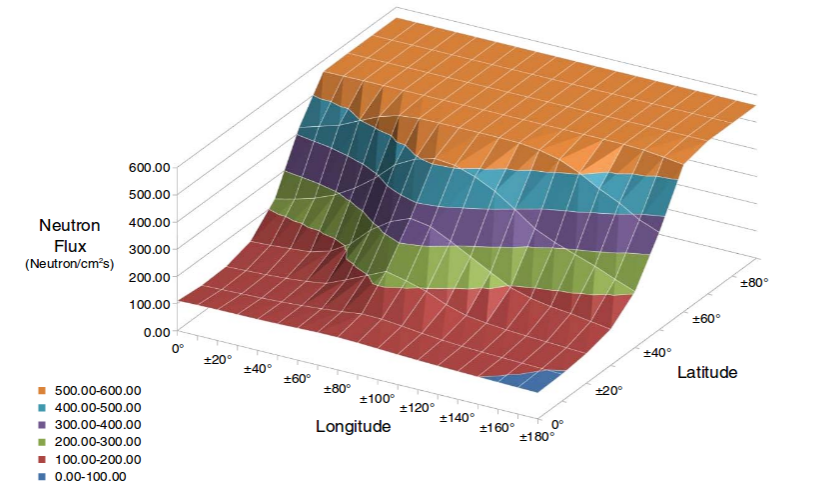
\includegraphics[scale=0.4]{figures/img/neutron-flux.png}
   \caption{Neutron Flux at 40,000 Feet.}
\label{fig:neu-flux}
\end{figure}





\section{Research Objectives}



The main objective of this project is to develop a faulty behaviour model for FPGA-based
circuits described at a high-level of abstraction.

By using neural networks, fault behaviour
models are developed and their accuracy is validated. The developed models could be used to
replace any component of the entire circuit with faulty versions of the components described
at a high-level of abstraction

The
goal of this research was to develop an approach for modeling the faulty behaviour of a
digital circuit in the presence of cosmic rays.

his ensures that the effect of faulty behaviour of each
component on a system could be analyzed at a high-level of abstraction and the mitigation
technique could be used to improve the robustness of more critical parts


The
goal of this research was to develop an approach for modeling the faulty behaviour of a
digital circuit in the presence of cosmic rays.


To implement effective high-level CR computer model one has to (a) design and implementation of the emulation system, (b) design and implementation of an experimental setup for bombardment,  c) feasible for aerospace system, and d) develop  a strategy to develop a high-level model from the results (signatures) derived from the emulation and bombardment setup. In the context of the development of a whole simulation methodology including CR environment and CR effects at
system and component levels, the objectives of this projects are:

\begin{itemize}
\item The goal of this work is to provide a fault injection platform flexible and optimized for
FPGA-based systems, allowing emulate configuration faults on SRAM-based FPGAs

\item Define CR environment in the context of future aircraft structures  at the level of electrical systems
\item Study existing databases of effects of CR at electrical systems level
\item Complete the analyses of the result of the CR characteristics recorded and derive the consequences in the aircraft embedded system
\item Develop the computer model of the CR effects
\item Simulate numerically the effect at component and electrical system level
\item Develop a strategy for evaluating the robustness of systems against CR
\item Propose update of CR requirements for electrical systems
\item Proposed the methodology and the models based on data observed in on-board experiments


\end{itemize}



The main challenges we foresee are:
\begin{itemize}
\item Development of the complex circuits and testing under radiation, e.g., soft-error analysis for sequential circuits
\item Make a model at higher-level of abstraction from the data extracted at lower level 
\item Experimental set-up for bombardment

\end{itemize}


  

\section{Novelty and Impact}


\begin{itemize}
\item The development and implementation of an early validation strategy at higher abstraction level helps to identify at what extent mitigation strategies are required
\item Study the system susceptibility under neutron-induced single even effect
\item Compare the neutron induced and proton induced errors
\item Signature for the sequential circuit
\item Computer model to study CR effects at early in the embedded system design
\end{itemize}


%%% Local Variables:
%%% mode: latex
%%% TeX-master: "../Document"
%%% End:
       % Introduction au sujet de recherche.
\Chapter{LITERATURE REVIEW \& PRIOR WORK}\label{sec:related}\selectlanguage{english}


This chapter is dedicated to the revision of some of the fundamental concepts and current research in different areas related to this project: radiation effects on SRAM-FPGAs, soft-error, hard-error. Fault-injection, SEUs, Signatures, and benchmarks for radation testing. All of these topics are equally relevant for the purpose of this research that, ideally, places itself as an attractive research project.

\section{Radiation Environment}

A Single Event Effect (SEE) results from a single energetic particle. When the particle strikes a sensitive node in a semi-conductor device, the ionization by the particle might produce a current pulse inside the device, which might cause soft or hard errors in the configurtaion memory of the device. Results in data corruption, transient disturbance, high current conditions (non-destructive and destructive
effects). SEE can if not handled well cause unwanted functional interrupts or in worst case catastrophic failures. Commonly, SEEs include single event upset (SEU), single event latch-up (SEL), single event burn-out (SEB), and single event transient (SET) etc as mentioned in Table~\ref{SEE-Summary}. SEEs may happen to electronic devices in these environments which is prune to the radiations. For example,
\begin{itemize}


   \item  Space (caused by space radiation)
    \item Air-plane (caused by atmospheric neutron)
    \item Close to nuclear reactor (caused by reaction neutron)
    \item Everywhere (IF caused by natural decay radiation in the materials of devices)

\end{itemize}



\begin{table}
\caption{Single Event Effects Summary}
\centering
\label{SEE-Summary}
\scalebox{0.4}{

   \begin{tabular}{c|c|c}
         \toprule
    \hline
     
     Single Event Upset (SEU)                  & corruption of the information \\ & stored in a memory element            & Memories, latches in logic devices                                  \\ \hline
    
    Multiple Bit Upset (MBU)                  & several memory elements \\ & corrupted by a single strike                & Memories, latches in logic devices                                  \\ \hline
    Single Event Functional Interrupt (SEFI) & corruption of a data path      & Complex devices with built-in state       \\ \hline
    Single Hard Error (SHE)                   & unalterable change of state in\\ & a memory element                     & Memories, latches in logic devices                                 \\ \hline
    Single Event Transient (SET)              & Impulse response of certain\\ & amplitude and duration                  & Analog and Mixed Signal circuits                      \\ \hline
    Single Event Disturb (SED)                & Momentary corruption of the\\&information stored in a bit             & combinational logic, latches in logic devices                       \\ \hline
    Single Event Latchup (SEL)                & high-current conditions                                              & CMOS, BiCMOS devices                                                \\ \hline
    Single Event Snapback (SESB)              & high-current conditions                                              & N-channel MOSFET, SOI devices                                       \\ \hline
    Single Event Burnout (SEB)                & Destructive burnout due to\\ & high-current conditions                  & BJT Power MOSFET    \\ \hline
    Single Event Gate Rupture (SEGR)         & Rupture of gate dielectric due\\&to high electrical field\\ & conditions & Power MOSFETs \\ \hline
    
    \bottomrule
    
    \end{tabular}
    }
\end{table}







\subsection{Neutrons Effects on FPGA}

FPGAs are complex reconfigurable devices that comprise a wide family of different resources. The basic structure of modern FPGAs includes interconnect resources, clock-management resources, configurable logic blocks (CLBs), input/output
blocks (IOBs), and embedded blocks such as digital signal processors (DSPs), general-purpose processors, high-speed IOBs, and memories. CLBs are used to perform simple
combinational and sequential logic. These blocks are typically formed of look-up tables
(LUTs), multiplexers, flip-flops, and carry logic. Programmable interconnect resources, such
as routing switches, allow interconnecting CLBs, IOBs and embedded blocks to implement multiple systems (Buell et al., 2007).
The logic and routing resources in an FPGA are controlled by the bits of a configuration memory, which may be based on either antifuse, flash, or SRAM technology. The
design flow of FPGA-based systems as shown in Figure~\ref{fig:fpga-struct} adapted from ~\cite{hauck2010reconfigurable} involves the creation of a bitstream to load into the
device.



\begin{figure}[tb!]
 \centering
  \captionsetup{justification=centering}    
   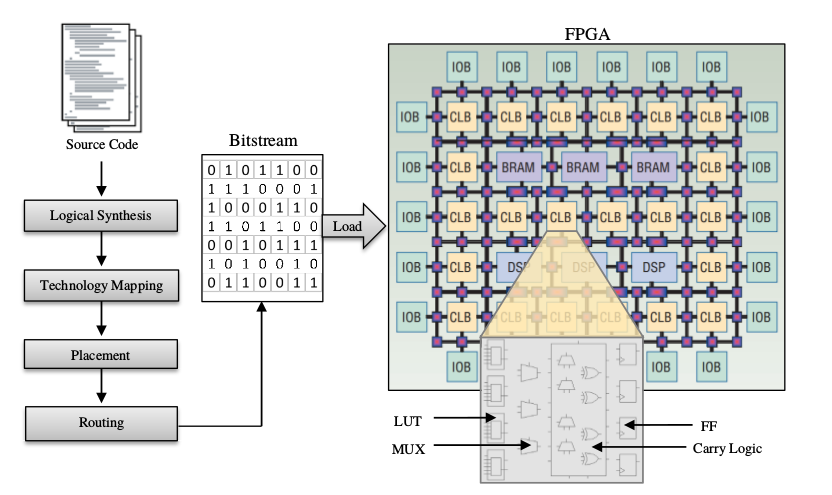
\includegraphics[scale=0.4]{figures/img/FPGA-structure.png}
   \caption{FPGA Structure and Design Flow}
\label{fig:fpga-struct}
\end{figure}



\subsection{Shielding Effect}

The process starts with the system design written
in a hardware description language (HDL), e.g., VHDL or Verilog. Next, the design is optimized and mapped into the FPGA’s available resources through logical synthesis,
technology mapping, placement, and routing. Finally, the generated bitstream downloaded into the device, and the device starts functioning according to the designer design.
Like any other semiconductor device, FPGAs are sensitive to radiation effects.
Mostly, these effects depend on the technology used to store the configuration data.
Regarding the impact of SEEs on reliability and functionality, FPGAs based on SRAM
technology are a particular class of devices. The foremost concern for SRAM-based FPGAs is
SEUs within the configuration memory. In such devices, this memory may represent more
than 80 percent of the total memory bits, increasing the probability of configuration faults.
Upset configuration bits may change the logic and routing of the implemented system, as
shown in Figure~\ref{fig:seu}, leading to functional failures in an unpredictable way. In contradiction, the primary concern for anti-fuse and flash-based FPGAs is SETs and SEUs within user flip-flops
and block memories. However, the configuration memory blocks of anti-fuse and flash-based
FPGAs offer a relative immunity to SEEs, but these devices have lower logic capacity and
cannot be reprogrammed an unlimited number of times, making SRAM-based FPGAs more
suitable for complex systems requiring frequent reconfiguration and adaptation~\cite{quinn2015validation, violante2004simulation}.

\begin{figure}
 \centering
  \captionsetup{justification=centering}    
   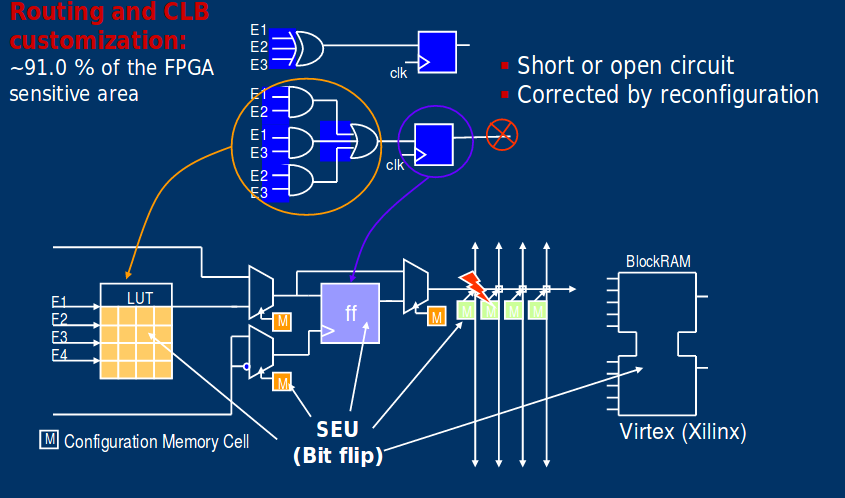
\includegraphics[scale=0.4]{figures/img/seu.png}
   \caption{Upset FPGA configuration bits may change the logic and routing.}
\label{fig:seu}
\end{figure}


\section{Faults Caused by Cosmic Rays in Digital Circuits}
\subsection{Single Event Effects Mechanism}
%\subsection{Faults, and Failure}


\section{Design Verification by Fault Injection}



As we discussed before, SRAM-based FPGAs are particularly sensitive to SEUs. The configuration memory is the most sensitive part, by changing the configuration memory, may affect the overall functionality of the system. The work have done so far deal the SEU effects on FPGAs, combines the simulation, radiation, and emulation testing~\cite{quinn2015validation, violante2004simulation, hobeika2014multi, robache2013methodology, quinn2015using, souari2015optimization}. These papers described how they make the faulty behavior of the system to build an accurate representation of the system. The work presented in~\cite{quinn2015using} described the benchmark that can be used for the reliability and radiation effects study on FPGAs and microprocessors. FPGAs offer high densities and run-time programmability facility make inconvenient to use in the aerospace domain. But, FPGAs are sensitive to high-energy ions.  We need to study the sensitivity of SRAM-based FPGAs to heavy ions that show the suitability and analysis of effects of radiation on FPGAs when employed in space, e.g., usage of FPGAs in aircraft. The work presented in~\cite{hobeika2014multi} investigate the sensitivity of SRAM-based FPGAs devices not only for the simulation-based approach but also used emulation and radiation testing for evaluating the effects of SEUs. The work presented in~\cite{souari2015optimization} described the fault injection emulation in Xilinx FPGA based on the identification of critical configuration bits. Based on SRAM-based FPGAs, two aspects can be considered:

\begin{itemize}


\item SEUs may alter the contents of a register in the data path, or the content of the state register.
\item SEUS may alter the content of the configuration memory.

\end{itemize}



\subsection{Simulation}

The work presented in~\cite{robache2013methodology} discuss the fault simulation, fault emulation, and radiation testing. Starting from the simulation, I can interrogate how the authors used the concept of signatures to capture and reproduce the faulty behavior due to SEUs very early in the design process.
Radiation testing is an expensive approach and requires a state-of-the-art facility. The alternative to the radiation testing is the fault-injection approach.  The work presented in~\cite{hobeika2014multi} described the concept of faulty behavior signature. The work demonstrates how faulty behavior signatures allow building high-level models, e.g., high-level faulty model, i.e., Simulink, that reflects the faulty behavior of a combinational circuit represented at gate-level  (injected with one fault arbitrarily selected from a fault list). The main contribution of this work is to capture the effects of radiations on a circuit modeled at a low abstraction level and then abstract it to a  higher level. This challenge can be accomplished by introducing the concept of faulty behavior signature.  The fault injection tool that is used named - LIFTING.  The purpose of this tool is to study the effects of different types of faults on a circuit at gate-level. The tool used the stuck-at 0 and 1 are injected in each node of the design. The LIFTING is a simulation-based gate-level fault injection tool that used the circuit netlist file, e.g.  *.v file, input test vectors, and fault parameters as inputs produced two output files. The one is the golden report and the second consist of fault injection report. These two outputs are used to generate the signatures.  The signature represents the compressed faulty behavior of the circuit. The signatures consist of arrays of errors and their probabilities of occurrence. The signatures are either arithmetic or logic.  The third step is to make a high-level model that corresponds the low-level circuit. The work presented in this paper helps to make a faulty block with Simulink that reads a signature and generates errors according to the distribution.

\subsection{Emulation}
The emulation of SEUs in an FPGA is done by flipping the bit in the configuration memory. The emulation can be done by using the IP provided by the Xilinx named - LogiCORE. The work adopted the emulation work also proposed in the~\cite{hobeika2013flight}.  The work described a completed automated methodology to emulate SEUs on an FPGA efficiently. The authors used the reconfigurable flight control system based on a reference adaptive control model. The difference between the work presented in~\cite{hobeika2014multi} and~\cite{hobeika2013flight} is that; in~\cite{hobeika2013flight} the authors used the flight control system that is based on a linear plant model. Whereas, in~\cite{hobeika2014multi}the emulation is performed on the circuits (adder and multiplier). The work presented in~\cite{hobeika2014multi} used the SEU controller. The emulation is the four step process.

\begin{itemize}

\item Identification of an emulation zone.
\item Fault list generation.
\item SEU emulation.
\item Result Analysis.

\end{itemize}



The identification of an emulation zone used the concept of the essential bits which can be extracted by the Xilinx BitGen command. For example, 253227 bits are identified as the total essential bits in~\cite{hobeika2013flight}, among them, 57464 belongs to the interested essential bits. The step is used to minimize the time because an FPGA device contains millions of configurable bits, emulating a bit flip for every cell would be time-consuming. BitGen gives only the essential bits; that
considered critical bits. The second step generates the fault list. This action creates a list of the corresponding bit addresses (exact bit position to be emulated).  For example, authors observed 7000 emulation requests in~\cite{hobeika2013flight}.  The third step used auto-correct mode in which one bit is flipped at a time and the detect-only mode  (bit flips accumulation possible) where bits are flipped without correction. In the final step, an in-house script is used to characterize and quantify the design sensitivity to SEUs. This script is used to compare the results with the faulty one and fault-free. Authors observed 638 total number of failure in~\cite{hobeika2013flight}. Similarly, authors observed 80384 essential bits among them 2454 are considered as the interested ones for the adder circuit, for multiplier interested essential bits are 1314 among 92337 total essential bits.
The emulation can be performed on the Virtex 5. The 16-bit adder and  8-bit-by-8-bit multiplier are used as a testing circuit. The signatures are recorded in the accumulation mode. And, the estimation of the critical bits performed in the auto-correct mode.
The Emulation setup presented in~\cite{souari2015optimization} adopted the approach for the estimation by fault injection based on the sensitivity. Authors proposed the method in which fault are injected based on the specific bits configurations defined according to their contents and the type of FPGA resources. This new approach outperformed the traditional random fault injection with speed up factors to two orders of magnitude. This fault injection method based on the prioritizing specific subsets of configuration bits. These configuration bits are classified with the statistical analysis according to their values (0 or 1, and 2). The SEU controller a macro developed by Xilinx assuring fault injection, detection, and correction is used a fault injection engine in their experiments. The fault injection is prioritized using the following three steps:

\begin{itemize}

\item   {Classification of the configuration bits into subsets.
        a.  Bits set to 1/0 of LUT.
        b. Bits set to 1/0 configuring other than LUT.
        c. Bits set to 1/0 configuring other resources not identified as  potentially critical by bitgen.}
        
        
\item  {Estimating the number of critical bits of the set by randomly injecting faults in the bits of each set. This method helps to find the most critical zones of the FPGA.}

\item {Prioritized the fault injection in the identified (step-2) most critical zones.
These classification steps are done with the help of EBC and EBD files provided by the bitgen. The experimental results presented in [5] evaluated the SEU sensitiveness as well as bitgen efficiency. The results are evaluated between random fault injection with different prioritized bit subsets.  The first observation authors concluded - the bitgen did not accurately identify all the critical bits meaning the bitgen limitations. Second authors did the prioritizing the most sensitive subset. It would involve exhaustive fault injection. The authors used fault injection to get an estimated number of critical bits as well as the related estimation error. They used the term critical bit error estimate (CBEE). The authors claimed the CBEE observed for the random approach is higher than the observed under the bits subsets.  The ratio of observed critical bits (ROCB) observed for the random injection is far less than the different bits subsets.}



\end{itemize}



\subsection{Radiation testing}
The hardware setup consists of two Artix-7 board. Board A used as a reference and board- B is subjected to radiations. The board-A is not bombarded, and it hosted the counters, reference design error detection and signature computation, memories to store signatures and communication controller. A total 20 runs performed on the adder and 14 on the multipliers. Arithmetic errors for both approached DSP and LUT are observed (151 vs. 291 for DSP). This is due to DSP strategy; SEUs can add registers in the data path, leading to the sequential type of errors. The authors in this work compare the results from the fault simulation, fault emulation, and radiation testing. The purpose is to express as signatures, intended to reproduce the faulty behavior. They showed that simulation and emulation based signatures could contain the same error values as obtained with radiation but their probability of occurrence could significantly different. The arithmetic signature for TRIUMF to emulation is 85.3 % for adder and 84.8% for the multiplier. Similarly, the matching with the simulation of adder and multiplier with TRIUMF is 84.8 % and 100 % respectively.



%\subsection{Stuck-at Fault Model}
%\subsection{Functional Fault Model}
%\subsection{Open Fault}
%\subsection{Stuck-On and Stuck-Off}


\section{Fault Models}


\subsection{Stuck-at Fault Model}

\subsection{Functional Fault Model}






%\subsection{Benchmark for Radiation Testing}
The suitable selection of the benchmark for the radiation testing of microprocessor and FPGAs is a recently topic of ongoing research. The benchmarks are used to evaluate the performance under different architectures, technology, and compiler. There is no such standard benchmark employed to study microprocessor and FPGAs under the effects of radiations; make it difficult to assess the changes in fabrication technology, architecture, and circuitry. The work presented in~\cite{quinn2015using}described the software and hardware benchmark under the neutron test data. The unavailability of the such a benchmark for testing because radiation hardness assurance techniques are applied only to circuit layouts or manufacturing process. There is no standard test circuits available, researcher, used flip-flop or D-latches to compare their results. In recent years, radiation effects community shown interest to develop a standard set of circuits that include complex and realistic algorithms and can be adapted to different FPGAs.  Currently, without standard benchmark researcher used the following approach for testing:

\begin{itemize}


\item Homemade Design.
\item Circuits from Opencore.
\item Proprietary designs.
\end{itemize}


The problem with this approach as no two organizations used the same set of codes or circuits, difficult to make the comparison. There is a need for collaboration to make a suitable set of benchmark for reliability application and study the effects of radiation under the same conditions. The criteria used to set a standard benchmark including:

Repeatability of benchmark tests.
A representative of deployed computing workload.
Availability of fixed input vectors.
Cross-platform implementation.
The ability to repeat test itself is an important part of the standardized testing. By repeating the algorithms, the input test vector, the compilation, the synthesis setting help researchers to have the enough information. It is necessary to provide a wide variety of realistic algorithms so that the system can be tested as likely to the realistic application. Defining the input test vector is an essential step because many hardware errors can be observed under the specific set of the test vector. It is an open question which input test vector should be adopted, under the specific set of criteria. Finally, the implementation of the algorithms in portable languages help to use the same set of codes on the different platform. For example, assembly language for the microprocessors limit the ability to compare and port codes on the different platform. But the hardware benchmark developed in VHDL can ease the problem; the same circuit can be ported to any FPGA.

\textbf{FPGA Radiation Benchmark}

The FPGA benchmark mentioned in this paper is ITC'99 which is well defined ATPG benchmark. This benchmark meets all the requirements, e.g., realistic algorithms, input vectors, scalability, and portability. The circuits are implemented in the HDL so that it can be ported to different FPGAs. The first 15 circuits from the ITC'99 are adopted for the benchmark as shown in Table I.

\textbf{Software Radiation Benchmark}

The software radiation benchmark is harder to design than the FPGA radiation benchmark. The development of the standard set of algorithm that can be ported on different architectures would be a challenging task e.g., porting an algorithm to 16-bit microcontroller to GPU. The authors are interested in the software benchmark where the computational load can be divided into the parallel processes or run on a single core. The commonly used software benchmark comprises of fast fourier transform, matrix multiplication and quick-sort algorithm as they are commonly used in many applications and useful for the evaluating the reliability of parallel processors. The software benchmark comprises the following code.

\begin{itemize}
\item AES-128;
\item Cache test;
\item FFT;
\item Hotspot;
\item HPCCG;
\item Matrix Multiply;
\item Quicksort
\end{itemize}





\textbf{Radiation Testing}
The radiation testing is completed at Los Almos Neutron Science Center (LANSCE). The results are provided for the microcontroller, ARM cores, GPUs, and FPGAs. The B13 from ITC99 is used under the hardware benchmark suite; Virtex- 5 is used as a hardware platform. They also provide the result for the mitigation. For mitigation, they used X-TMR and VERI-Place. The failure in time (FIT) are decreased under mitigation, but the overhead is increased (circuit area increased).

\textbf{Hardware Benchmark Testing}
For the hardware radiation testing the authors used the B13 from the ITC’99 benchmark suite. The circuit is too small so it can be replicated 30 times, the implementation is done on the Virtex-5. Both unmitigated and mitigated version are tested. The results for FPGA radiation reports SDCs from the mitigated circuits normalized to the SDCs from the unmitigated circuits. Mitigated circuits are likely to fail at three times the rate of the unmitigated circuit, because of the increased size of the circuit from the mitigation process. The mitigated circuit cross-section is three times larger than an unmitigated circuit when SEUs accumulate. The authors conclude; the VERI-place mitigated circuits perform better than the X-TMR mitigated circuits.

\textbf{Software Benchmark Testing}
Software benchmark radiation testing is done on the flash-based microcontroller,  a ferroelectric-memory-based microcontroller, two ARMs, and GPUs. These components are tested with both mitigated and unmitigated codes. The results reported in the paper for two different microcontroller and two ARMs cores. For microprocessors: these microprocessors have very small SRAM the FITs are very small. In some cases, there is no error from the code during many days of testing. They also implemented the matrix multiplication, FFT, and Hotspot on NVIDIA K20 GPU and applied mitigation methods (ECC, ABFT, and DWC).  The purpose is to see the effect of overhead by applying the mitigation technique; the overhead has been increased as compared it with the unhardened configuration.
In short, the work presented in [3] evaluate a common set of hardware and software benchmarks to evaluate reliability and radiation effects on FPGA and microprocessors.





%\section{Fault-detection, mitigation and correction in the FPGA }


The impact of SEUs on SRAM FPGA devices has been studied in~\cite{bellato2004evaluating}. Many  techniques  have  been  proposed to provide highly reliable FPGA devices, e.g. radiation-hardened FPGAs~\cite{rockett2007radiation}, in-order to lower the effect of radiation-induced SEUs. However, radiation-hardened  SRAM  FPGAs  typically have  a  low  density, and  they  only  may  lower  the  probability of SEUs to occur but  not  completely avoid  them. Therefore, non radiation-hardened FPGAs, like the  Xilinx Kintex-7, are evaluated under a harsh radiation  environment~\cite{wirthlin2014soft}. Even on radiation-hardened FPGAs, the SEU rate in a low-earth orbit flight experiment can be up to 16 events per day~\cite{quinn2012orbit}. A wide  variety  of  SEU  fault  mitigation  techniques  for SRAM-based  FPGAs  have  been  proposed  during  the  past years. These techniques can be categorized into module redundancy techniques such as triple modular redundancy (TMR)~\cite{lyons1962use} and techniques that use scrubbing of the FPGA configuration memory~\cite{heiner2009fpga}. Also the combination of  both techniques has been shown to be able to increase the reliability of FPGA modules significantly ~\cite{ostler2009sram}. FPGA-based TMR approaches replicate a given module which shall be protected either statically or dynamically~\cite{angermeier2011runtime}. The different granularities of voted replicas  are evaluated in~\cite{bolchini2007tmr}. However, no upset rates and consequential no reliability figures are provided. Nevertheless, TMR techniques are  known to often cause an excessive and unacceptable overhead in terms of power  consumption and area. Since the intensity of a cosmic rays is not constant but may vary over several magnitudes depending on the solar activity, a worst-case radiation protection is far too expensive in most cases. A self-adaptive system is proposed in~\cite{glein2014self}, which monitors the current SEU rate and exploits the opportunity of partial reconfiguration of FPGAs to implement redundancy such as TMR on demand. 

Memory scrubbing is a well-known correction technique for the configuration memory of SRAM-based FPGAs. It consists on re-writing the configuration memory after the FPGA is configured to restore its original content. It is often a transparent operation for the running application. This is possible because modern FPGAs offer a dynamic partial reconfiguration (DPR) feature. The circuit that enables the scrubbing is commonly named scrubber. Additionally, readback is the process of reading the configuration memory of the FPGA after it is configured. Both processes (readback and scrubbing) can be used to implement different scrubbing methodologies as shown in~\cite{herrera2013design}. Scrubbing can be implemented using an internal or external interface as shown in~\cite{berg2008effectiveness}. When external interface is used, the scrubbing logic is implemented outside the FPGA. In the case of Xilinx FPGAs several external interfaces are available; however, the Select MAP interface has the highest data throughput. On the other hand, there is only one internal interface named ICAP~\cite{xilinx}. This internal interface can be accessed from the reconfigurable logic of the FPGA and it is a replica of the Select MAP interface. Also scrubbers can be implemented in software or hardware. The scrubbing process can be implemented using a microprocessor with the advantage of a high flexibility to implement different complex scrubbing methodologies but with lower configuration speeds and lower energy efficiency.

\section{Faults Behavioural Modeling}

%\subsection{Built-In Self-Test (BIST)}
%\subsection{All Test Pattern Generator (ATPG)}
%\subsection{Scan Chain Testing}

\section{Conclusion}
The work done so far [1, 2, 3, 4, and 5] evaluated and quantified the SEU effects by performing simulation, emulation, and radiation on an SRAM-based FPGA. Implemented a design, observed its faulty behavior in the presence of SEU and extracted the corresponding fault model. Presented an automated methodology to efficiently used the SEU controller. Discussed the fault injection on the specific subsets rather than random and discussed the selection of the suitable benchmark for FPGA and microprocessor radiations. 




%%% Local Variables:
%%% mode: latex
%%% TeX-master: "../Document"
%%% End:
  % Revue de littérature.
\Chapter{PROPOSED APPROACH}\label{sec:approach}\selectlanguage{english}

This chapter is dedicated to the methodology that we propose to exert to achieve the objectives of this research project, i.e. Methodology and Algorithms for High-level Modelling of Cosmic Radiations Impacts on Electrical Systems. First of all, we will identify four main research axes: (1)  Fault emulation platform for sequential circuits to generate signatures; (2) radiation-based experiments; (3) high-level modeling to study radiation impacts on electrical systems; and (4) Simulator- isoneo.

In addition to the development of our research along these axes, we also have a plan to implement a technology demonstrator on FPGA and, fly in an aircraft, e.g., \textbf{CMC BEE platform}.

\section{Research Axis 1: Measuring Sequential Circuit Testing and Reliability}

\subsection{Emulation Environment and Framework}
\subsection{Sequential Circuit Fault Injection Mechanism}
\subsection{Sequential Circuit Test Generation}


\section{Research Axis 2: Modeling of Sequential Circuit}
\subsection{Modeling of Sequential Circuit with Model Checking}

\subsection{Modeling of Sequential Circuit with BDD/ADD}

\subsection{Modeling of Sequential Circuit with Monte-carlo Techniques}

\subsection{Modeling of Sequential Circuit with Markovian-Chain Analysis}



%The fault injection platform proposes for this project emulates SEUs, more specifically single-bit upsets (SBUs) within the configuration memory of SRAM-based FPGAs. We will study the effects of SEU on sequential circuits, and introduce a  framework for analyzing and detecting them. We will do the modeling and analysis of sequential circuits susceptibility to soft errors. Accurate sequential SEU estimation requires capturing the mechanism of error propagation and masking at both combinational and sequential levels. The challenging task for the sequential circuits under SEUs: the difference between sequential and combinational circuits from the context of ATPG and single stuck-at fault model. In this project, we will concentrate on sequential synchronous circuits. The problem we will face and encounter that the controllability of auxiliary inputs and observability of secondary outputs for the sequential circuits.  We will study and implement a technique which eases sequential circuits testing and ATPG by making controllability and observability much simple.
%
%\subsection{Fault Injection}
%
%We need to examine the behavior of a design under faults. For fault injection there are two strategies: (a) \textit{Software based fault injection}, and (b) \textit{FPGA based fault injection}. 
%
%\begin{itemize}
%
%\item Two methods will develop for software based fault injection. First, the source HDL code is modified to allow fault injection. Second, the simulation tool is used to force the error injection during simulation. 
%\item For FPGA-based simulation, we will use single error mitigation core from Xilinx~\cite{xilinx}. The idea is to integrate this core with our system to generate a modified bitstreams to emulate the occurrence of errors. We will use this strategy.
%\end{itemize}





\section{Research Axis 3: Radiation Bombardment}
This part of the project is a neutron-induced Single Event Effect test in a commercial FPGA from Xilinx. The primary objective is to investigate the radiation effects reliability for the critical application. We will implement the sequential circuit and data acquisition system. The results we want to achieve to drive signatures for the sequential circuits. Our focus is on the analyzing the impact of multiple errors in state flip-flops, during the cycles following the cycle when faults occur. The following milestones we want to achieve from radiation bombardment experiment.

\begin{itemize}
\item Modeling of SEU, MBU and analyzing their effect on logic circuits.
\item Evaluation of changes in error rates due to SEUs in sequential circuits.
\item Compute the error probability, and signatures from bit-upsets can vary for different outputs and different circuits. 
\item Evaluation of the impact of multiple flip-flop upsets in sequential circuits.
\item Determining the outputs that are most susceptible to errors due to faults in logic.
\item Determining the parts of the circuit (gates or gate clusters) that have the largest impact on circuit error probability.
\item Estimation of lower and upper bounds of circuit susceptibility to transient.
\end{itemize} 
%
%\section{Research Axis 3: High-level Modelling}
%
%To model and analyze the sequential circuit susceptibility to soft errors, we need to used the approximate methods, e.g.,
%\begin{itemize}
%
%\item Binary Decision Diagram and Algebraic decision diagram.
%\item Markov-chain analysis based error rate estimation, which can provide steady-state Single-Error rate estimates following a hit. 
%\item A  Monte Carlo for SEU Analysis of Sequential Circuits based on the probability of the bit-flips and estimates the states outputs and signatures.
%
%\end{itemize}
%\subsection{Simulator}
%
%We also have a plan to develop a simulator with the help of \textit{isoneo}. The simulator is based on the Matlab / Simulink models. The simulator takes the input a parameterization file corresponding to the operational architecture of the system. This file is generated from the configurator; it is in XML format.
%From this configuration, the simulator initially initializes a model of the system failure tree.
%This model is then exploited dynamically during the simulation phase to evaluate the level of reliability of the system and its components. The simulator executes the simulation model with the constraints and concludes a level of safety for each equipment and the global system.

\section{Optional Research Axis: Fault Mitigation}
Fault-mitigation can be achieved in two ways: preventing faults from happening and
recovering after their occurrence. Fault preventing is achieved by using hardened components and/or shielding. But fault preventative is not a viable solution in terms of a project cost. More complex fault-mitigation methodologies can be implemented at the architectural level. We need to develop some fault-mitigation strategies like triple module redundancy with  dynamic reconfiguration of the hardware~\cite{jacobs2012reconfigurable} and/or something like the work presented in 
%Jacobs \emph{et al.}~\cite{jacobs2012reconfigurable} and Alderighi \emph{et al.}~\cite{violante} promote the use of SRAM-FPGAs for reconfigurable fault-tolerant space applications.
~\cite{jacobs2012reconfigurable} used fault tolerance framework (RFT) that enables system designers to dynamically adjust a system's level of redundancy and fault mitigation based on the varying radiation incurred at different orbital positions. Notably, the reconfigurable fault tolerance framework in~\cite{jacobs2012reconfigurable} is based on an upset rate modeling tool that used to capture time-varying radiation effects in a given orbit.


\section{Project Plan}


\textbf{Summary}

\textbf{Phase  01:} The emulation platform will be the starting point of research. We will use the SEUs for the configuration memory upsets. Selection of a suitable benchmark, which is probably ITC'99~\cite{ITC}used for the testing purpose. We will evaluate the bits sensitivity as well. We will implement the prototype. 

\textbf{Phase  02:} Evaluate the experimental setup under the neutron radiation at Triumf.


\textbf{Phase 03:} Develop an efficient methodology and high-level model for soft-error of sequential circuits, i.e., Monte-Carlo sampling, approximate approaches, symbolic methods for efficient estimation. The simulator development will keep with all these three phases.



%\section{Timetable}
%The development of the tasks identified in Chapter~\ref{sec:approach}, and the most important milestones of this project are presented in Figure~\ref{timetable}.
%In our intentions, the design of a time predictable computer architecture, the development of novel timing analysis techniques, and the FPGA prototypes implementation will unfold as a series of sequential tasks with relatively small interleaving. Dependability and real-time requirements, on the other hand, should be kept in mind throughout the whole advancement of the project.
%
%\begin{figure}[h]
%\centering
%\begin{tikzpicture}
%\begin{ganttchart}[
%x unit=0.36cm,
%y unit title=1.0cm,
%y unit chart=1.5cm,
%%vgrid,
%hgrid,
%inline,
%]{1}{48}
%\gantttitle{Research Project}{48} \\
%\gantttitle{2016}{12} \gantttitle{2017}{12} \gantttitle{2018}{12} \gantttitle{2019}{12}\\
%
%
%
%\ganttbar[bar height=.4]{Literature Review and Comp .Exam}{6}{24}\\
%%\ganttmilestone[]{Comp. Exam}{20}\\
%%\ganttmilestone[]{AHS}{6}
%%\ganttmilestone[]{TODAES}{12}\\
%\ganttbar[bar height=.4]{Emulation Platform for Seq. ckt}{6}{35} \\
%\ganttbar[bar height=.4]{Radiation Experiment}{13}{24} \\
%\ganttbar[bar height=.4]{Modelling and Simulator}{25}{42} \\
%%\ganttmilestone[]{TAAS}{30}\\
%%\ganttbar[bar height=.4]{Novel Timing analysis techniques}{22}{38} \\
%%\ganttmilestone[]{DAC}{36}\\
%%\ganttbar[bar height=.4]{FPGA Implementation}{27}{38} \\
%%\ganttmilestone[]{TRETS}{40}\\
%\ganttbar[bar height=.4]{Tech. Demo.}{35}{42} \\
%%\ganttmilestone[]{IAC}{44}\\
%\ganttbar[bar height=.4]{Thesis Writing}{35}{46}
%%\ganttmilestone[]{Thesis}{44}\\
%%\ganttbar[bar height=.4]{The \emph{PolyOrbite} Project}{1}{44} 
%
%%\ganttlink{elem0}{elem1}
%%\ganttlink{elem0}{elem2}
%%\ganttlink{elem0}{elem3}
%
%%\ganttlink{elem3}{elem4}
%
%%\ganttlink{elem5}{elem6}
%%\ganttlink{elem5}{elem7}
%
%%\ganttlink{elem7}{elem8}
%\end{ganttchart}
%\end{tikzpicture}
%\caption{Timetable.}
%\label{timetable}
%\end{figure}









         
\Chapter{PRELIMINARY RESULTS}\label{sec:preliminary}\selectlanguage{english}

In this chapter, we present the preliminary results of this research work. These results are focused on the implementation of a probabilistically analysable instruction and data cache for the Ion MIPS32 processor on
FPGA. We developed a random placement and replacement policy that fulfills
all the requirements for PTA. Our experiments show that the cache fulfills all the requirements for PTA, and program timing can be determined with arbitrary accuracy. In addition, random placement and replacement improve the observed WCET from 6\% to 19\% w.r.t. a Least Recently Used policy.



\section{Relative Sensitivity Based Emulation}

This paper presents an FPGA implementation of a probabilistically analyzable
cache inspired by the simulation work presented
in~\cite{Kosmidis:2013:CDP:2485288.2485416}. In this paper we have
kept the same approach for the cache behaviour:
\begin{enumerate}
\item The cache uses a random replacement policy
\item The cache uses a parametric random placement policy based on
 a hash function
\item The cache placement is deterministic for each benchmark execution, but
  randomized across executions
\item We measure end-to-end execution time for a series of benchmarks
\end{enumerate}

\section{High-Level Fault Model}
\section{Sequential Circuits Fault model}
%\section{Hardware Implementation}
\label{Hardware Implementation}

%\subsection{Cache RTL Model}
\label{Cache Model}

We implemented an instruction and data cache for the Ion
MIPS32 processor~\cite{ION}. A completely novel, configurable cache
design was implemented in VHDL and integrated with the Ion core. The
cache is completely configurable (bus width, size, block size,
policies, etc.) with VHDL generics and could be easily ported to other
processor designs. Figure~\ref{fig:cache-structure} shows the main components of our design:

\begin{figure}
 \centering
  \captionsetup{justification=centering}    
   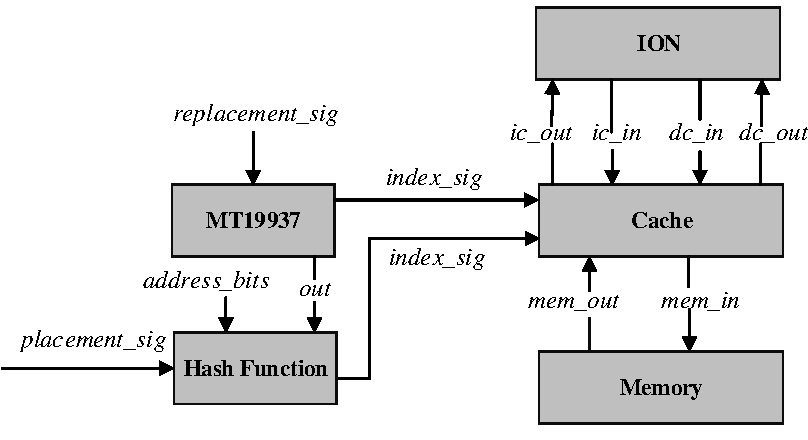
\includegraphics[scale=0.2]{figures/img/cache_structure_c.pdf}
   \caption{Structure of the proposed cache.}
\label{fig:cache-structure}
\end{figure}

\begin{enumerate}
\item The cache block contains the cache memory proper, as well as the
logic to manage the replacement policy (random and least-recently-used)
\item A hash function block that operates on the index signal to the
  cache, randomizing the mapping between memory blocks and cache blocks
\item A pseudo-random number generator (MT19937)
\item The Ion core, which provides a MIPS32 ISA and controls the whole
  system
\end{enumerate}

Our cache has three fundamentally novel features that enable probabilistic
timing analysis:
\begin{enumerate}
\item A random \textbf{placement} policy which uses a parametric hash
  function to shuffle the initial placement of blocks in the cache memory
\item A random \textbf{replacement} policy that uses high-quality random
numbers to provide statistically-verifiable guarantees that replacement
events are uniformly distributed among the available cache blocks
\item A high-quality pseudo-random number generation, with an extremely
long period, to generate random bits for the implementation of the cache
random policies
\end{enumerate}
%
%
%\subsection{Random Number Generation}

In our cache design, we used the Mersenne Twister algorithm to
generate random numbers. In particular, we used the MT19937 algorithm,
which is considered as a good hardware solution for a random number
generation~\cite{Matsumoto:1998:MTE:272991.272995}. MT19937 provides a
uniform pseudo number pattern with a period of
$2\textsuperscript{19937-1}$, with a width of 32 or 54 bits.  We used
the OpenCores implementation of MT19937~\cite{OpenCores}. The
synthesis report shows that the maximum clock frequency the design can
achieved is 147.016 MHz, with a throughput of 30 Msamples per second.

%\subsection{Parametric Hash Function}
%\label{PHF}
%
%The idea of using a parametric hash function for the implementation of
%random placement was given
%by~\cite{Kosmidis:2013:CDP:2485288.2485416}. This design is remodelled
%for this work, replacing their Multiply With Carry (MWC) random number
%generator with the MT19937, increasing the quality of the random
%numbers as well as the period.  The redesign was driven by the fact
%that MWC does not pass some statistical normality
%tests~\cite{bandyopadhyay2015discrete}, and its period might be
%insufficient for long running
%applications~\cite{Goresky:2003:EMR:945511.945514}.
%
%Standard placement assigns sets to cache lines based on the index bits
%of the memory address. If the placement policy assigns two memory
%addresses to the same cache set, they will systematically be in conflict. 
%To deal with this deterministic nature while randomizing the timing
%behaviour of the placement policy, we use a parametric hash
%function with a random number as an input.  A random number
%provides a unique and constant cache set mapping for each address.
%If the random number changes, the cache set in which the address is mapped changes. By changing random number only at a new execution, programs can be analyzed with end-to-end runs assuming that the cache is initially empty.
%Figure~\ref{fig:hash_function} shows the structure of the hash function.
%
%








%\subsection{Random Number Generation}
%
%In our cache design, we used the Mersenne Twister algorithm to
%generate random numbers. In particular, we used the MT19937 algorithm,
%which is considered as a good hardware solution for a random number
%generation~\cite{Matsumoto:1998:MTE:272991.272995}. MT19937 provides a
%uniform pseudo number pattern with a period of
%$2\textsuperscript{19937-1}$, with a width of 32 or 54 bits.  We used
%the OpenCores implementation of MT19937~\cite{OpenCores}. The
%synthesis report shows that the maximum clock frequency the design can
%achieved is 147.016 MHz, with a throughput of 30 Msamples per second.

%\subsection{Parametric Hash Function}
\label{PHF}


\begin{figure}[t!]

 \centering
  \captionsetup{justification=centering}    
   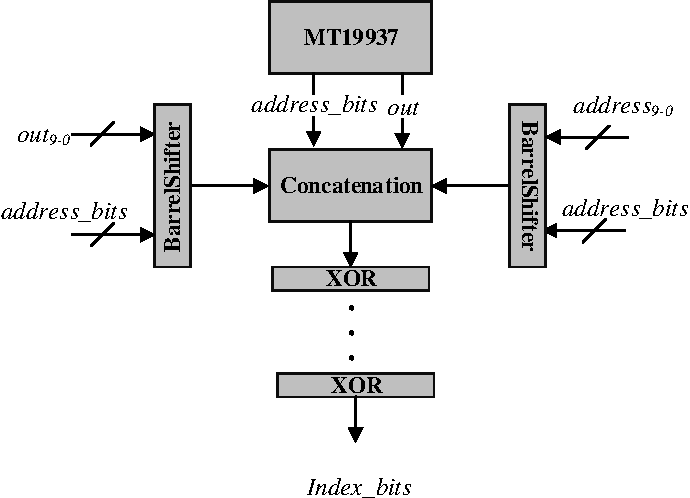
\includegraphics[scale=0.8]{figures/img/hash_function.pdf}
   \caption{The hash function uses a random number, the address bits, and four XOR stages to produce a random placement.}
\label{fig:hash_function}
\end{figure}



%\begin{figure}[t!]
%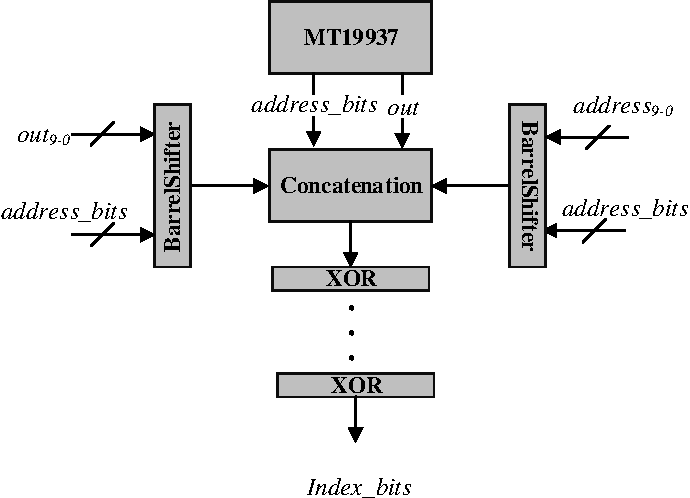
\includegraphics[width=\columnwidth]{figures/img/hash_function.pdf}
%\caption{The hash function uses a random number,
%the address bits, and four XOR stages to produce a random placement}
%\label{fig:hash_function}
%\end{figure}

The idea of using a parametric hash function for the implementation of
random placement was given
by~\cite{Kosmidis:2013:CDP:2485288.2485416}. This design is remodelled
for this work, replacing their Multiply With Carry (MWC) random number
generator with the MT19937, increasing the quality of the random
numbers as well as the period.  The redesign was driven by the fact
that MWC does not pass some statistical normality
tests~\cite{bandyopadhyay2015discrete}, and its period might be
insufficient for long running
applications~\cite{Goresky:2003:EMR:945511.945514}.

Standard placement assigns sets to cache lines based on the index bits
of the memory address. If the placement policy assigns two memory
addresses to the same cache set, they will systematically be in conflict. 
To deal with this deterministic nature while randomizing the timing
behaviour of the placement policy, we use a parametric hash
function with a random number as an input.  A random number
provides a unique and constant cache set mapping for each address.
If the random number changes, the cache set in which the address is mapped changes. By changing random number only at a new execution, programs can be analyzed with end-to-end runs assuming that the cache is initially empty.
Figure~\ref{fig:hash_function} shows the structure of the hash function.






%



%\section{Experimental Results}

\begin{table}[t]
\caption{Resource utilization and overhead (Virtex-5)}
\label{resource_table}
\begin{center}
\begin{tabular}{llllll}
\toprule
              & LRU & \multicolumn{3}{c}{RND} & Overhead \\
\cmidrule(lr){3-5}
              &   &  Cache & Hash	& MT19937 &  \\
\midrule
%Available     & 69120    &       69120   & 69120           \\
LUT Flip Flop  & 1904    &  1792   &  656   &  117  & 34.7\% \\ 
Slice LUTs     & 6026    &  5637   &  660   &  419  & 11.6\%  \\
%BRAMs          & 4       &  6      &  2     &  1    & 225\%\\
\bottomrule
\end{tabular}
\end{center}
\end{table}


\begin{figure}[t!]

 \centering
  \captionsetup{justification=centering}    
   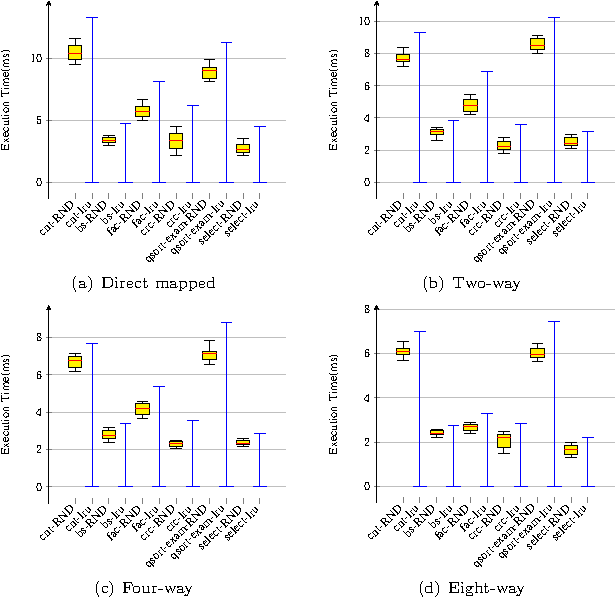
\includegraphics[scale=0.8]{figures/img/boxplot.pdf}
   \caption{Execution Time Measurement}
\label{fig:boxplot}
\end{figure}
The architecture used in our experiments is the OpenCores Ion MIPS32
processor. We integrated both an I-cache and a D-cache, and we
implemented the whole system on the Xilinx ML505 FPGA evaluation
board, using the XC5VLX110T chip using  Xilinx ISE-14.4 and ModelSim 10.1.a. We used two separate 4~kB cache
memories for data and instructions, both with a 32-byte line size.  To
evaluate our design, we used M\"alardalen real-time benchmark~\cite{mrtc:bench} suite. We selected six benchmarks: \textit{cnt, bs,
  fac, crc, qsort-exam and select}. These benchmarks use arrays
and matrices, and have nested loops structures which are ideal to test
our design~\cite{Competitive}. We omitted those benchmarks using
external libraries and unstructured code to simplify the
software implementation and data collection. 



Each benchmark was run on multiple cache configurations profiles, and
we derived its execution time profile using MBPTA, with 30 runs per
profile to approximate a normal error distribution.
To show that our cache generates identically distributed execution times (as
required for PTA), we used the Kolmogorov-Smirnov test~\cite{books/daglib/0020904},
which shows that the null hypothesis (the data are normally distributed) cannot
be rejected for all benchmarks at the 5\% confidence level ($p>0.062$).
We compared our results (RND) with a standard Least-Recently-Used (LRU)
cache policy implementation.

Figures \ref{fig:boxplot} show the timing
distributions for all benchmarks on our cache from direct-mapped to
8-way associative, respectively. As an added advantage, our random
cache shows a 19\% improvement in worst case execution time w.r.t to
LRU for a direct-mapped cache, 11\% for 2-way cache, 8\% for a 4-way
cache, and 6\% for an 8-way cache. As expected, LRU gets closer to RND
as the number of ways increases: the number of conflict miss is
greatly reduced by additional ways.

\section{Conclusion}
In this paper, we present the RTL model of a randomized L1 data and
instruction cache. This cache uses a high-quality random number
generator for random placement and replacement. Random placement is
obtained with a parametric hash function that shuffles the association
between memory addresses and cache blocks. The cache is integrated
with the Ion MIPS32 processor, and verified to generate independent
and identically distributed timing events, such that Measurement-Based
Probabilistic Timing Analysis is possible (MBPTA). We test our cache
and MBPTA approach on a variety of benchmark from the M\"alardalen
benchmark suite and show a noticeable improvement (5-15\%) in terms of
measured Worst Case Execution Time (WCET) as well as enabling the
identification of safe probabilistic WCET (pWCET) bounds.  Future work
will consider the implementation of shared randomized caches for
multi-core architectures.
         
\Chapter{CONCLUSIONS}\label{sec:conclusions}\selectlanguage{english} 

In this proposal, we have demonstrated our research will be focused on investigation of a design, methodologies, and implementation of a time predictable fault tolerant computing system evaluated by the probabilistic timing analysis (PTA). As our target domain is a real-time industry. We will stress the importance of a worst case execution time (WCET) estimation.
Nowadays, the investigations of new timing analysis techniques are an unavoidable need because of the growing complexity of a modern embedded computers and the aerospace industry will especially a benefit from the introduction of a such technologies in terms of  reliability and design costs. Our approach will leverage probabilistic approach to enable the timing analysis in computing systems.
As a consequence, this research has a potential to make computing systems smarter, more reliable, and easier to design and to program. At the same time, we think that our results will make decisive steps ahead in a fairly unexplored research area - integration of fault-tolerance techniques in time predictable computer architecture.


In our preliminary results, we showed that how probabilistically analysable cache can be integrated in a MIPS processor to make the foundation for a probabilistically analysable computing systems. The research published in~\cite{NEWCAS} proved the effectiveness of a measurement based probabilistic timing analysis (MBPTA). Furthermore, our most recent results demonstrated that probabilistic timing technique is a promising approach for the future timing analysis of a real-time aerospace embedded system.

Through this research, we hope to be able to have an impact on how computer engineers and system designers will think of probabilistic computing in near future, and contribute to create the next generation of a real-time embedded systems for aerospace industry.
We will target field-specific international  journals such as the ``ACM Transactions on Real-time  Systems'' and the ``ACM Transactions on Reconfigurable Technology and Systems'', or conferences including tracks dedicated to the automated design of embedded systems, such as the ``Design Automation Conference'' and the ``Design, Automation \& Test in Europe'' conference.

\section{Work Breakdown Structure}
Figure~\ref{wbs} presents the work breakdown structure (WBS) of our research project. At level 2 of this tree chart, we identify four groups of tasks: the ones related to the acquisition of knowledge; those related to the development of new knowledge; an experimental phase; and, finally, project management tasks.

Knowledge acquisition includes the class work done towards the credit requirements of the PhD program and the review of the scientific literature. 

The knowledge extension task can be split along the four research axes defined in Chapter~\ref{sec:approach}. The experimental phase goes from the definition of a test plan to the experimental evaluation of our prototype on a CubeSat  platform.

Project management tasks involve the writing of conference and journal articles, as well as the preparation of a thesis and its defense.

\begin{figure}[h]
\vspace{2cm}
\centering
\begin{tikzpicture}[
  level 1/.style={sibling distance=40mm},
  edge from parent/.style={->,draw},
  >=latex]

% root of the the initial tree, level 1
\node[root, fill = black!30] {Research Project}
% The first level, as children of the initial tree
  child {node[level 2,fill = black!10] (c1) {Knowledge Acquisition}}
  child {node[level 2,fill = black!10] (c2) {Knowledge Extension}}
  child {node[ level 2,fill = black!10] (c3) {Experimental Phase}}
  child {node[level 2,fill = black!10] (c4) {Project\\ Management}};

% The second level, relatively positioned nodes
\begin{scope}[every node/.style={level 3}]
\node [rounded corners,fill = white, below of = c1, xshift=15pt] (c11) {\footnotesize Classes};
\node [rounded corners,fill = white, below of = c11] (c12) {\footnotesize Literature\\ Review};

\node [rounded corners,fill = white, below of = c2, xshift=15pt] (c21) {\footnotesize PTA};
\node [rounded corners,fill = white, below of = c21] (c22) {{\footnotesize Predictable computing}};
\node [rounded corners,fill = white, below of = c22] (c23) {\footnotesize Fault tolerance};
\node [rounded corners,fill = white, below of = c23] (c24) {\footnotesize Reconfiguration.};
\node [rounded corners,fill = white, below of = c24] (c25) {\footnotesize Multicore Architecture.};

\node [rounded corners,fill = white, below of = c3, xshift=15pt] (c31) {\footnotesize Design};
\node [rounded corners,fill = white, below of = c31] (c32) {\footnotesize Algorithm Eval.};
\node [rounded corners,fill = white, below of = c32] (c33) {\footnotesize FPGA Implementation.};
\node [rounded corners,fill = white, below of = c33] (c34) {\footnotesize Tech. Demo.};

\node [rounded corners,fill = white, below of = c4, xshift=15pt] (c41) {\footnotesize Conferences};
\node [rounded corners,fill = white, below of = c41] (c42) {\footnotesize Journals};
\node [rounded corners,fill = white, below of = c42] (c43) { \footnotesize Thesis and\\ Graduation};
%\node [fill = black!30, below of = c43] (c44) {Thesis and\\ Graduation};

\end{scope}

% lines from each level 1 node to every one of its "children"
\foreach \value in {1,2}
  \draw[->] (c1.195) |- (c1\value.west);

\foreach \value in {1,...,5}
  \draw[->] (c2.195) |- (c2\value.west);

\foreach \value in {1,...,4}
  \draw[->] (c3.195) |- (c3\value.west);

\foreach \value in {1,...,3}
  \draw[->] (c4.195) |- (c4\value.west);
\end{tikzpicture}
\caption{Work breakdown structure.}
\label{wbs}
\end{figure}

\newpage
\section{Timetable}
The development of the tasks identified in Chapter~\ref{sec:approach}, and the most important milestones of this project are presented in Figure~\ref{timetable}.
In our intentions, the design of a time predictable computer architecture, the development of novel timing analysis techniques, and the FPGA prototypes implementation will unfold as a series of sequential tasks with relatively small interleaving. Dependability and real-time requirements, on the other hand, should be kept in mind throughout the whole advancement of the project.

\begin{figure}[h]
\centering
\begin{tikzpicture}
\begin{ganttchart}[
x unit=0.36cm,
y unit title=1.0cm,
y unit chart=1.5cm,
%vgrid,
hgrid,
inline,
]{1}{48}
\gantttitle{Research Project}{48} \\
\gantttitle{2015}{12} \gantttitle{2015}{12} \gantttitle{2016}{12} \gantttitle{2017}{12}\\



\ganttbar[bar height=.4]{Literature Review}{1}{16}\\
%\ganttmilestone[]{Comp. Exam}{20}\\
%\ganttmilestone[]{AHS}{6}
%\ganttmilestone[]{TODAES}{12}\\
\ganttbar[bar height=.4]{Leon 3 processor analysis}{13}{32} \\
\ganttbar[bar height=.4]{Architectural Modifications}{17}{32} \\
\ganttbar[bar height=.4]{Probabilistic component design}{18}{38} \\
%\ganttmilestone[]{TAAS}{30}\\
\ganttbar[bar height=.4]{Novel Timing analysis techniques}{22}{38} \\
%\ganttmilestone[]{DAC}{36}\\
\ganttbar[bar height=.4]{FPGA Implementation}{27}{38} \\
%\ganttmilestone[]{TRETS}{40}\\
\ganttbar[bar height=.4]{Tech. Demo.}{35}{42} \\
%\ganttmilestone[]{IAC}{44}\\
\ganttbar[bar height=.4]{Thesis Writing}{35}{46}
%\ganttmilestone[]{Thesis}{44}\\
%\ganttbar[bar height=.4]{The \emph{PolyOrbite} Project}{1}{44} 

%\ganttlink{elem0}{elem1}
%\ganttlink{elem0}{elem2}
%\ganttlink{elem0}{elem3}

%\ganttlink{elem3}{elem4}

%\ganttlink{elem5}{elem6}
%\ganttlink{elem5}{elem7}

%\ganttlink{elem7}{elem8}
\end{ganttchart}
\end{tikzpicture}
\caption{Timetable.}
\label{timetable}
\end{figure}





%%%
%%%  SYNTHESE DES TRAVAUX
%%%
%\section{Synthèse des travaux}
%Texte.
%
%%%
%%%  LIMITATIONS
%%%
%\section{Limitations de la solution proposée}\label{sec:Limitations}
%
%%%
%%%  AMELIORATIONS FUTURES
%%%
%\section{Améliorations futures}
%Texte.
         % Conclusion.
%\backmatter
%\renewcommand\bibname{RÉFÉRENCES}
\renewcommand\bibname{REFERENCES}
\bibliography{Document}
\bibliographystyle{polymtl}  % Format de la bibliographie.
%
%\ifthenelse{\equal{\AnnexesPresentes}{O}}{
%\appendix%
%\newcommand{\Annexe}[1]{\annexe{#1}\setcounter{figure}{0}\setcounter{table}{0}\setcounter{footnote}{0}}%
%%%
%%  Annexes.
%%
%%  Note: Ne pas modifier la ligne ci-dessous.
\addcontentsline{toc}{compteur}{ANNEXES}
%%
%%
%%  Toutes les annexes doivent être inclues dans ce document
%%  les unes à la suite des autres.
\Annexe{DÉMO}
Texte de l'annexe A\@. Remarquez que la phrase précédente se termine
par une lettre majuscule suivie d'un point. On indique explicitement
cette situation à \LaTeX{} afin que ce dernier ajuste correctement
l'espacement entre le point final de la phrase et le début de la
phrase suivante.


\begin{landscape}
\Annexe{ENCORE UNE ANNEXE}
Texte de l'annexe B\@ en mode «landscape».
\end{landscape}

\Annexe{UNE DERNIÈRE ANNEXE}
Texte de l'annexe C\@.
}{}
\end{document}
